\begin{center}
\Huge
Folkeskolens afgangsprøve i gymnasiet
\end{center}
Vi skal i dag arbejde med folkeskolens afgangsprøve, men hvor vi har lavet opgaverne om til, hvordan de kunne se ud, hvis vi ville møde dem i gymnasiet. Vi arbejder med folkeskolens afgangsprøve fra maj 2022. Den første af opgaverne er opgaven, som I møder den i folkeskolens afgangsprøve og den anden del af opgaven er opgaven, som I ville møde den i gymnasiet. I kan
ikke nødvendigvis regne med, at opgaverne er helt ens. 

\subsubsection*{Uden hjælpemidler}

\begin{center}
	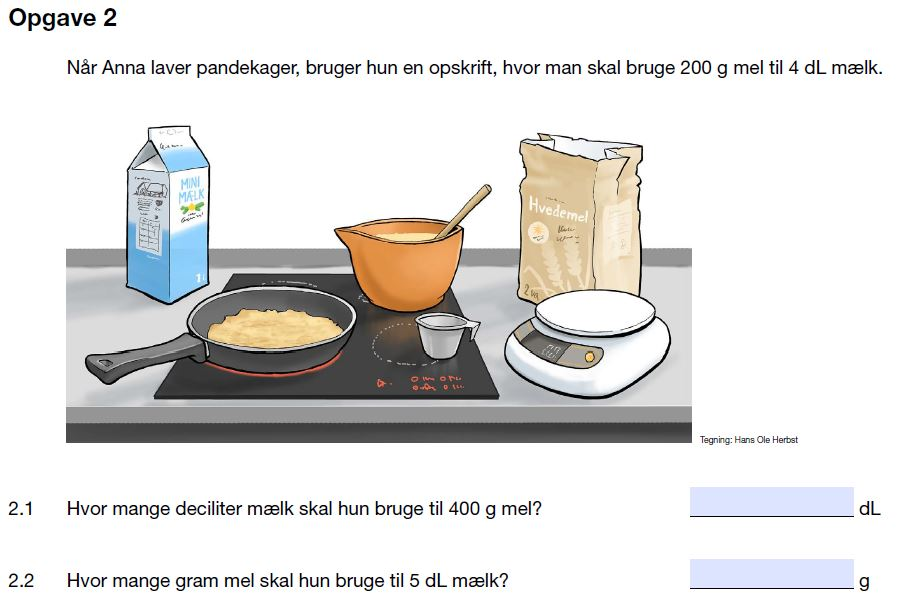
\includegraphics[width = 0.8\textwidth]{Billeder/opg2fsk}
\end{center}

\begin{opgavetekst}{Opgave 2}
	I en pandekageopskrift skal der bruges 200g mel til 4 dL mælk.
\end{opgavetekst}

\begin{delopgave}{}{1}
	Afgør, hvor meget mel, der skal bruges til per dL mælk i opskriften og opstil en model, der
	beskriver mængden af mel, der skal bruges i opskriften som funktion af mængden af mælk. 
\end{delopgave}
\begin{delopgave}{}{2}
	Brug din model til at afgøre hvor meget mælk, der skal bruges til 400g mel.
\end{delopgave}
\begin{delopgave}{}{3}
	Brug din model til at afgøre hvor meget mælk, der skal bruges til 4dL mælk. 
\end{delopgave}

\begin{center}
	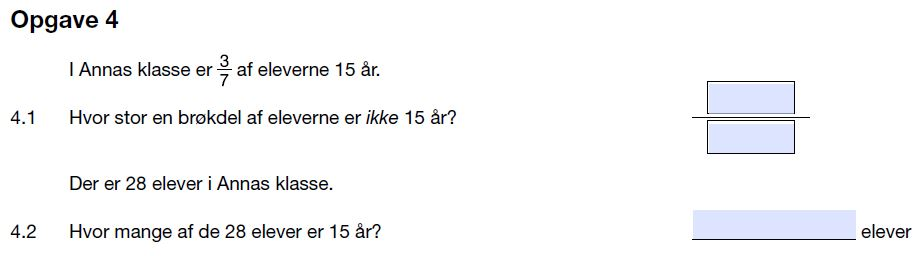
\includegraphics[width= 0.8\textwidth]{Billeder/opg4fsk}
\end{center}

\begin{opgavetekst}{Opgave 4}
	Udregn følgende:
\end{opgavetekst}

\begin{delopgave}{}{1}
	$1-\frac{3}{7}$.
\end{delopgave}
\begin{delopgave}{}{2}
	$28\cdot \frac{3}{7}$.
\end{delopgave}

\newpage
\begin{center}
	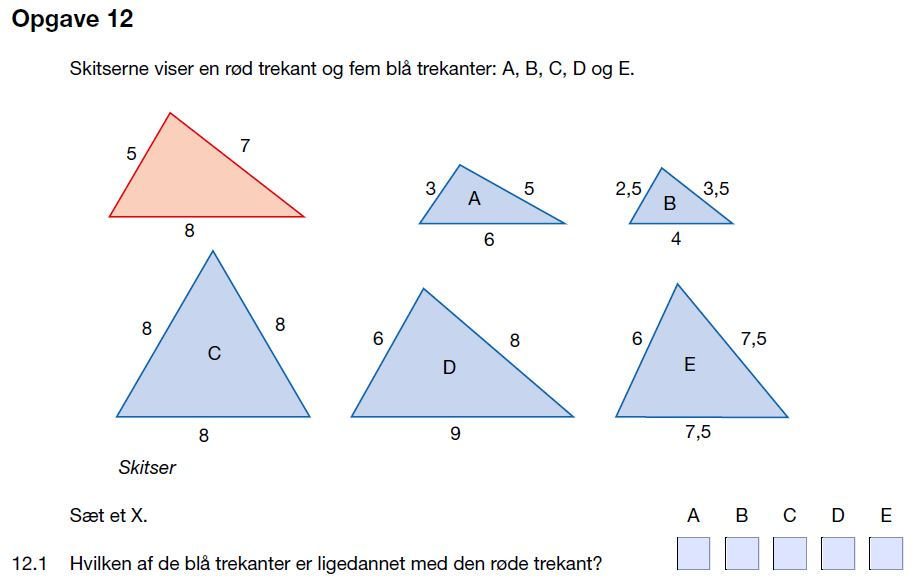
\includegraphics[width = 0.8\textwidth]{Billeder/opg12fsk}
\end{center}

\begin{opgavetekst}{Opgave 12}
	To trekanter $A$ og $B$ er ligedannede. Den længste af siderne i $A$ har en sidelængde 
	på 8 og den længste af siderne i $B$ har en sidelængde på 4. De resterende af sidelængderne
	i $A$ er 5 og 7. 
\end{opgavetekst}
\begin{delopgave}{}{1}
	Bestem de resterende sidelængder i $B$. 
\end{delopgave}
\begin{delopgave}{}{2}
	Afgør, om trekant $B$ er retvinklet. 
\end{delopgave}


\newpage

\begin{center}
	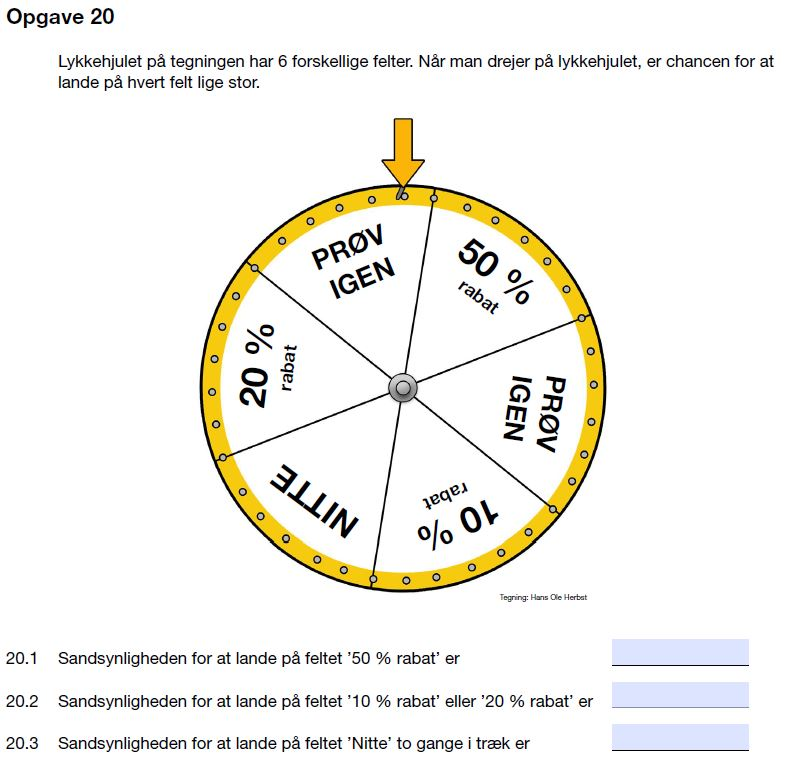
\includegraphics[width = 0.8\textwidth]{Billeder/opg20fsk}	
\end{center}

\begin{opgavetekst}{Opgave 20}
	Et eksperiment har udfaldsrummet $\{1,2,3,4,5,6\}$, og sandsynligheden for hvert af 
	udfaldene fremgår af Tabel \ref{tab:ssh}.
	\begin{table}[H]
		\centering
		\begin{tabular}{c|c|c|c|c|c|c}
			Udfald & 1 & 2 & 3 & 4 & 5 & 6 \\
			\hline
			Sandsynlighed & $0.1$ & $0.25$ & $0.1$ & $0.15$ & $0.2$ & $0.2$ 
		\end{tabular}		
		\caption{Sandsynligheder for eksperiment}
		\label{tab:ssh}
	\end{table}
	\phantom{h}
\end{opgavetekst}

\begin{delopgave}{}{1}
	Bestem sandsynligheden for at få udfaldet enten 3 eller 4.
\end{delopgave}
\begin{delopgave}{}{2}
	Vis, at sandsynlighederne sammenlagt giver 1.
\end{delopgave}
\begin{delopgave}{}{3}
	Bestem sandsynligheden for at få enten 5 eller 6 to gange i træk.
\end{delopgave}

\newpage

\subsubsection*{Med hjælpemidler}

\begin{center}
	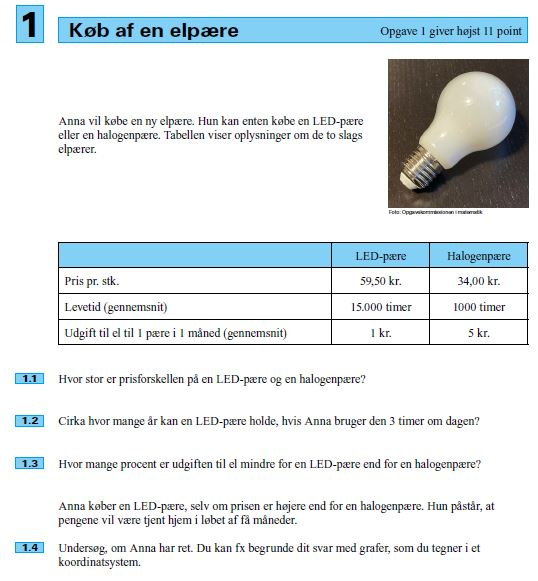
\includegraphics[width = 0.8\textwidth]{Billeder/opg1fskhj}
\end{center}
\begin{opgavetekst}{Opgave 1}
	En halogenpære koster månedligt 5kr at holde tændt. Den koster desuden 34kr at købe. 
\end{opgavetekst}

\begin{delopgave}{}{1}
	Opstil en model, der beskriver sammenhængen mellem antal måneder, halogenpæren har været 
	brugt, og prisen den koster at bruge. 
\end{delopgave}

\begin{delopgave}{}{2}
	Brug din model til at afgøre, hvor meget det koster at bruge pæren i et år.
\end{delopgave}

\begin{meretekst}
	Det oplyses, at prisen for at bruge en LED-pære kan beskrives ved modellen
	\begin{align*}
		p(x) = x + 59.50,
	\end{align*}
	hvor $p$ er prisen for at bruge pæren, og $x$ er antal måneder, den har været i brug.
\end{meretekst}

\begin{delopgave}{}{3}
	Tegn de to modeller i et koordinatsystem og brug modellernes forskrift til at afgøre, 
	hvornår LED-pæren bliver billigere end halogenpæren. 
\end{delopgave}

\newpage

\begin{center}
	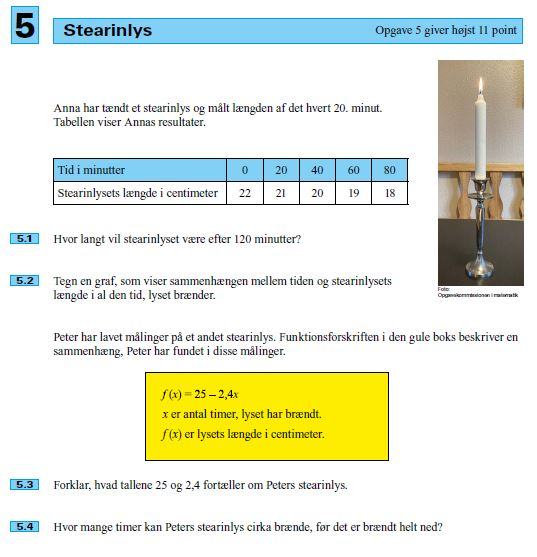
\includegraphics[width = 0.8\textwidth]{Billeder/opg6fskhj}
\end{center}

\begin{opgavetekst}{Opgave 6}
	Af Tabel \ref{tab:stearin} fremgår sammenhængen mellem et stearinlys længde i cm, 
	og hvor længde lyset har brændt.
	\begin{table}[H]
		\centering		
		\begin{tabular}{c|c|c|c|c|c}
		Tid i minutter & 0 & 20 & 40 & 60 & 80\\
		\hline
		Længde i cm & 22 & 21.1 & 19.8 & 19.2 & 18.0	
		\end{tabular}	
		\caption{Længde af stearinlys}
		\label{tab:stearin}
	\end{table}
	Det oplyses, at sammenhængen mellem tiden $x$ i minutter og længden af stearinlyset $f$ kan 
	beskrives ved en funktion med forskriften
	\begin{align*}
		f(x) = ax + b.
	\end{align*}
\end{opgavetekst}

\begin{delopgave}{}{1}
	Brug tallene fra Tabel \ref{tab:stearin} til at bestemme en forskrift for $f$. 
\end{delopgave}

\begin{delopgave}{}{2}
	Brug $f$ til at afgøre, hvor langt stearinlyset vil være efter 120 minutter. 
\end{delopgave}

\begin{meretekst}
	Længden af et andet stearinlys kan beskrives af funktionen $g$ givet ved
	\begin{align*}
		g(x) = 25-2.4x,
	\end{align*}
	hvor $x$ er antal timer, lyset har brændt, og $g$ er lysets længde. 
\end{meretekst}


\begin{delopgave}{}{3}
	Forklar, hvad tallene 25 og 2.4 fortæller om stearinlyset
\end{delopgave}

\begin{delopgave}{}{4}
	Bestem hvor længe de to lys kan brænde, før de er brændt helt ned. 
\end{delopgave}
